% !TEX root =../ECE343_Slides_Rogers.tex

\begin{frame}{}
\renewcommand{\arraystretch}{1}
	\begin{textblock}{14}(0.5,1.75)
	\def\myfontsize{footnotesize}
	\setcounter{mylnum}{24}
%\def\myfontsize{normalsize}
\begin{center}
\begin{\myfontsize}
\begin{tabular}{| c | l | c | l |}
\hline
\textbf{Lesson} 		  	& \textbf{Topics}             & \pbox{5cm}{\textbf{Reading}}	& \textbf{Notes}		\\ \hline\hline
\ifnum\lessonNum=\value{mylnum} \rowcolor{green!20!white}\fi
	\themylnum  
	& BVP (Capacitor, Coax), Electric Potential	
	& 5.16
	&  LO 5.3  
\stepcounter{mylnum}\\ \hline \hline
\ifnum\lessonNum=\value{mylnum} \rowcolor{green!20!white}\fi
	\themylnum 	
	& Electric Boundary Conditions
	& 5.18-5.22	
	& LO 5.4			
\stepcounter{mylnum}\\ \hline
\ifnum\lessonNum=\value{mylnum} \rowcolor{green!20!white}\fi
	\themylnum 	
	& BC's/Capacitance			
	& 5.23-5.24
	& 	
\stepcounter{mylnum}\\ \hline
\ifnum\lessonNum=\value{mylnum} \rowcolor{green!20!white}\fi
	\themylnum 	
	& Electrostatic Lab			
	& Lab packet
	& 	
\stepcounter{mylnum}\\ \hline
\rowcolor{gray!20!white}\multicolumn{4}{| c |}{\textbf{Chapter 6: Steady Current \& Conductivity}}	\\ \hline\hline
\ifnum\lessonNum=\value{mylnum} \rowcolor{green!20!white}\fi
	\themylnum 	
	& Current density, Conductivity, Resistance
	& Ch. 6
	&   					
\stepcounter{mylnum}\\ \hline\hline
\rowcolor{gray!20!white}\multicolumn{4}{| c |}{\textbf{Chapter 7: Magnetostatics}}						\\ \hline\hline
\ifnum\lessonNum=\value{mylnum} \rowcolor{green!20!white}\fi
	\themylnum 	
	&  Magnetic Fields, Gauss' Law for Magnetism	
	& 7.1-7.3		
	&LO 7.1-7.2 \textbf{GR 2} 				
\stepcounter{mylnum}\\ \hline
\ifnum\lessonNum=\value{mylnum} \rowcolor{green!20!white}\fi
	\themylnum 	
	& Ampere's Law 	
	& 7.4-7.5, 7.9
	& LO 7.3		
\stepcounter{mylnum}\\ \hline 
\ifnum\lessonNum=\value{mylnum} \rowcolor{green!20!white}\fi
	\themylnum 	
	&  Ampere's Law Applied
	&  7.6-7.8
	& LO 7.3
\stepcounter{mylnum}\\ \hline 
\ifnum\lessonNum=\value{mylnum} \rowcolor{green!20!white}\fi
	\themylnum	
	& Magnetic Boundary Conditions	
	& 7.10-7.14	
	& LO 7.4 		
\stepcounter{mylnum}\\ \hline 
\ifnum\lessonNum=\value{mylnum} \rowcolor{green!20!white}\fi
	\themylnum  
	& Magnetostatics Lab
	& Lab packet
	&  		
\stepcounter{mylnum}\\ \hline \hline
\rowcolor{gray!20!white}\multicolumn{4}{| c |}{\textbf{Chapter 8: Time-Varying Fields}}					\\ \hline\hline
\ifnum\lessonNum=\value{mylnum} \rowcolor{green!20!white}\fi
	\themylnum 	
	& Faraday's Law, Displacement Current, Maxwell Eqns
	& 8.3, 8.8, 8.9
	& LO 8.1
\stepcounter{mylnum}\\ \hline 
\ifnum\lessonNum=\value{mylnum} \rowcolor{green!20!white}\fi
	\themylnum	
	& Faraday's Law, Displacement Current, Maxwell Eqns 
	&  8.3, 8.8, 8.9
	& LO 8.2-8.3
\stepcounter{mylnum}\\ \hline 

\rowcolor{gray!20!white}\multicolumn{4}{| c |}{\textbf{Chapter 9: Plane Waves in Lossless Media}}					\\ \hline\hline
\ifnum\lessonNum=\value{mylnum} \rowcolor{green!20!white}\fi
	\themylnum	
	& Maxwell's Equations in lossless, source-free region		
	& 9.1-9.2
	& LO 9.1	 
\stepcounter{mylnum}\\ \hline
\ifnum\lessonNum=\value{mylnum} \rowcolor{green!20!white}\fi
	\themylnum	
	& Maxwell's Equations in lossless, source-free region		
	& 9.1-9.2
	& LO 9.1	 
\stepcounter{mylnum}\\ \hline
%\ifnum\lessonNum=\value{mylnum} \rowcolor{green!20!white}\fi
%	\themylnum	
%	& Flex day
%	& 
%	& \textbf{GR 3}			 					
%\stepcounter{mylnum}\\ \hline 
\ifnum\lessonNum=\value{mylnum} \rowcolor{green!20!white}\fi
	\themylnum	
	& Uniform Plane Waves \& Polarization
	& 9.4-9.6
	& LO 9.2-9.3			
\stepcounter{mylnum}\\ \hline 
\ifnum\lessonNum=\value{mylnum} \rowcolor{green!20!white}\fi
	\themylnum	
	& Normal Incidence
	& Vol 2, 5.6-5.7
	&  LO 9.4-9.5
\stepcounter{mylnum}\\ \hline 
\ifnum\lessonNum=\value{mylnum} \rowcolor{green!20!white}\fi
	\themylnum	
	& Oblique Incidence			
	& Vol 2, 5.6-5.7
	& LO 9.5
\stepcounter{mylnum}\\ \hline 
\ifnum\lessonNum=\value{mylnum} \rowcolor{green!20!white}\fi
	\themylnum	
	& Oblique Incidence			
	& Vol 2, 5.6-5.7
	& LO 9.5
\stepcounter{mylnum}\\ \hline 
\ifnum\lessonNum=\value{mylnum} \rowcolor{green!20!white}\fi
	\themylnum	
	& Incidence Lab			
	& TBD
	& LO 9.5
\stepcounter{mylnum}\\ \hline 
%\ifnum\lessonNum=\value{mylnum} \rowcolor{green!20!white}\fi
%	\themylnum	
%	& Wrapup
%	& 
%	& 		 					
%\stepcounter{mylnum}\\ \hline 

\end{tabular}			
\end{\myfontsize}
\end{center}

	\end{textblock}
\end{frame}

%%%%%%%%%%%%%%%%%%%%%%%%%%%%%%%%%%%%%%%%%%%%%%%%%%%%%
%%%%%%%%%%%%%%%%%%%%%%%%%%%%%%%%%%%%%%%%%%%%%%%%%%%%%

\def\obja{ I can use the Biot-Savart law to simple magnetostatic systems to find the magnetic field at an observation point.}
\def\objb{  I can articulate the meaning of both the integral form and point form of Gauss' Law for magnetism.}
\def\objc{I can use Ampere's Law to calculate the magnetic field at an observation point for simple magnetostatic systems.}
\def\objd{  I can apply the magnetic field boundary conditions to calculate magnetic fields on both sides of a material boundary.  }
\begin{frame}{Ch 7 Learning Objectives}
	\begin{textblock}{14}(0.5,2.5)
	\begin{myblock}[0.95]{}
	\begin{small}
	\begin{enumerate}[{7}.1]
		\ifnum\objNum=1
			\item \alert{ \obja }
		\else 
			\item \obja
		\fi 
		\ifnum\objNum=2
			\item \alert{ \objb }
		\else 
			\item \objb
		\fi 
		\ifnum\objNum=3
			\item \alert{ \objc }
		\else 
			\item \objc
		\fi 
		\ifnum\objNum=4
			\item \alert{ \objd }
		\else 
			\item \objd
		\fi 	
	\end{enumerate}
	\end{small}
	\end{myblock}
	\end{textblock}
\end{frame}

%%%%%%%%%%%%%%%%%%%%%%%%%%%%%%%%%%%%%%%%%%%%%%%%%%%%%
%%%%%%%%%%%%%%%%%%%%%%%%%%%%%%%%%%%%%%%%%%%%%%%%%%%%%
\section{Boundary Conditions}
\begin{frame}{Magnetic Boundary Conditions}
\begin{textblock}{14.5}(0.5,3)
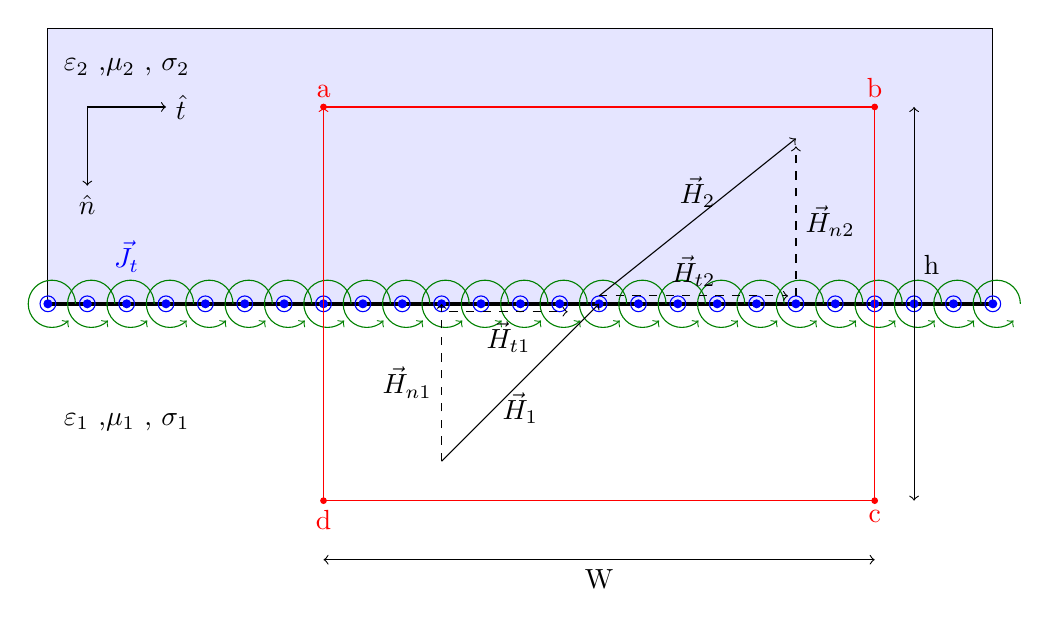
\begin{tikzpicture}

	\draw[fill=blue!10!white] (0,0) rectangle (12,3.5);
	\draw[ultra thick, black] (0,0) --++ (12,0);
	\node at (1,3) {$\varepsilon_2$ ,$\mu_2$ , $\sigma_2 $};
	\node at (1,-1.5) {$\varepsilon_1$ ,$\mu_1$ , $\sigma_1 $};
	
	% line charges
	\foreach \x in{0,0.5,1,...,12}{
		\draw[blue] (\x,0) circle (1mm);
		\draw[blue, fill=blue] (\x,0) circle (0.5mm);
		\draw[green!50!black, ->] (\x+0.35,0) arc (0:315:0.3);
	}
	\node[blue] at (1,0.6) {$\vec{J}_t$};
		
	% unit vectors
	\draw[->] (0.5,2.5) --++ (1,0) node[right] {$\hat{t}$};
	\draw[->] (0.5,2.5) --++ (0,-1) node[below] {$\hat{n}$};
	
	% material 2
	\draw[->] (5,-2) --++ (2,2) node[midway, below] {$\vec{H}_1$}; 
	\draw[->, dashed] (5,-2) --++ (0,2) node[left, midway] {$\vec{H}_{\text{n1}}$};
	\draw[->, dashed] (5.1,-0.1) --++ (1.5,0) node[below, midway] {$\vec{H}_{\text{t1}}$};
	
	% material 1
	\draw[->] (7, 0.1)  --++ (2.5,2) node[midway, above] {$\vec{H}_{2}$};
	\draw[->, dashed] (9.5, 0.1) --++ (0,1.9) node[right, midway] {$\vec{H}_{\text{n2}}$};
	\draw[->, dashed] (7,0.1) --++ (2.4,0) node[above, midway] {$\vec{H}_{\text{t2}}$};
	
	%contours
	\coordinate (a) at (3.5, 2.5);
	\coordinate (b) at (10.5, 2.5);
	\coordinate (c) at (10.5, -2.5);
	\coordinate (d) at (3.5, -2.5);	
	
	\draw[red, fill=red] (a) circle (1pt) node[above]  {a};
	\draw[red, fill=red] (b) circle (1pt) node[above]  {b};
	\draw[red, fill=red] (c) circle (1pt) node[below] {c};
	\draw[red, fill=red] (d) circle (1pt) node[below] {d};
	
	\path[draw=red, ->] (a) -| (b) -| (c) -| (d) -| (a);
	\draw[<->] (3.5,-3.25) --++ (7,0) node[midway, below] {W};
	\draw[<->] (11,2.5) --++(0,-5) node[pos=0.4, right] {h};
	%\draw[red, thick,->] (3.5,2.5) node[above left] {a} --++ (7,0) node[above right] {b} --++ (0,-5) node[below right] {c} --++ (-7,0) node[below left] {d} --++ (0,5);
\end{tikzpicture}

\end{textblock}
\end{frame}

%%%%%%%%%%%%%%%%%%%%%%%%%%%%%%%%%%%%%%%%%%%%%%%%%%%%%%
%%%%%%%%%%%%%%%%%%%%%%%%%%%%%%%%%%%%%%%%%%%%%%%%%%%%%%
\section{Transverse}
\begin{frame}{$\vec{H}$ Boundary Conditions: Transverse }
\begin{textblock}{7.5}(0.5,3)
\scalebox{0.5}{
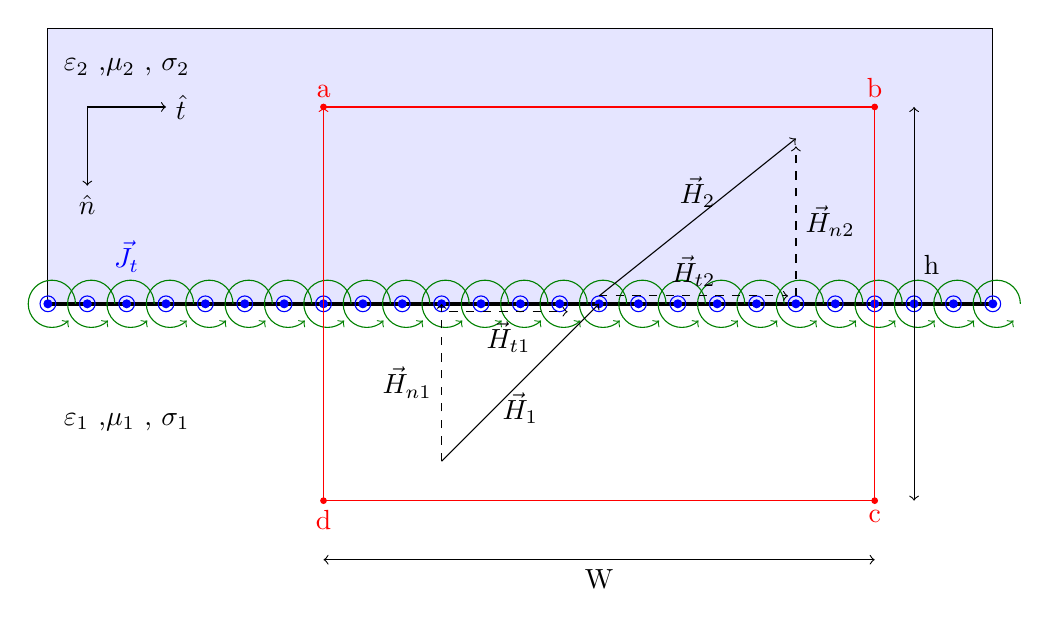
\begin{tikzpicture}

	\draw[fill=blue!10!white] (0,0) rectangle (12,3.5);
	\draw[ultra thick, black] (0,0) --++ (12,0);
	\node at (1,3) {$\varepsilon_2$ ,$\mu_2$ , $\sigma_2 $};
	\node at (1,-1.5) {$\varepsilon_1$ ,$\mu_1$ , $\sigma_1 $};
	
	% line charges
	\foreach \x in{0,0.5,1,...,12}{
		\draw[blue] (\x,0) circle (1mm);
		\draw[blue, fill=blue] (\x,0) circle (0.5mm);
		\draw[green!50!black, ->] (\x+0.35,0) arc (0:315:0.3);
	}
	\node[blue] at (1,0.6) {$\vec{J}_t$};
		
	% unit vectors
	\draw[->] (0.5,2.5) --++ (1,0) node[right] {$\hat{t}$};
	\draw[->] (0.5,2.5) --++ (0,-1) node[below] {$\hat{n}$};
	
	% material 2
	\draw[->] (5,-2) --++ (2,2) node[midway, below] {$\vec{H}_1$}; 
	\draw[->, dashed] (5,-2) --++ (0,2) node[left, midway] {$\vec{H}_{\text{n1}}$};
	\draw[->, dashed] (5.1,-0.1) --++ (1.5,0) node[below, midway] {$\vec{H}_{\text{t1}}$};
	
	% material 1
	\draw[->] (7, 0.1)  --++ (2.5,2) node[midway, above] {$\vec{H}_{2}$};
	\draw[->, dashed] (9.5, 0.1) --++ (0,1.9) node[right, midway] {$\vec{H}_{\text{n2}}$};
	\draw[->, dashed] (7,0.1) --++ (2.4,0) node[above, midway] {$\vec{H}_{\text{t2}}$};
	
	%contours
	\coordinate (a) at (3.5, 2.5);
	\coordinate (b) at (10.5, 2.5);
	\coordinate (c) at (10.5, -2.5);
	\coordinate (d) at (3.5, -2.5);	
	
	\draw[red, fill=red] (a) circle (1pt) node[above]  {a};
	\draw[red, fill=red] (b) circle (1pt) node[above]  {b};
	\draw[red, fill=red] (c) circle (1pt) node[below] {c};
	\draw[red, fill=red] (d) circle (1pt) node[below] {d};
	
	\path[draw=red, ->] (a) -| (b) -| (c) -| (d) -| (a);
	\draw[<->] (3.5,-3.25) --++ (7,0) node[midway, below] {W};
	\draw[<->] (11,2.5) --++(0,-5) node[pos=0.4, right] {h};
	%\draw[red, thick,->] (3.5,2.5) node[above left] {a} --++ (7,0) node[above right] {b} --++ (0,-5) node[below right] {c} --++ (-7,0) node[below left] {d} --++ (0,5);
\end{tikzpicture}
} % end scalebox

Using Ampere's Law for magnetism:
\visible<0|handout:1>{
\alert{
\eq{
	&\oint_C \vec{H} \mycdot \vec{d\ell} = \myi{encl} \\
} % end eq
} % end alert
} % end visible
\end{textblock}
\begin{textblock}{7}(8.5,2.5)
We can write:
\begin{scriptsize}
\visible<0|handout:1>{
\alert{
\eq{
	\circled{1}\; & \oint_C \vec{H} \mycdot \vec{d\ell}  = \int_a^d \vec{H} \mycdot\vec{d\ell}_1 + \int_d^c \vec{H} \mycdot\vec{d\ell}_2 \\[-4pt]
	&\qquad\qquad +  \int_c^b \vec{H} \mycdot\vec{d\ell}_3 +  \int_b^a\vec{H} \mycdot\vec{d\ell}_4 \\[-4pt]
	&= 0 + \int_d^c \vec{H} \mycdot\vec{d\ell}_2 + 0 +  \int_b^a\vec{H} \mycdot\vec{d\ell}_4 \\[-4pt]
	& =  \int_d^c \vec{H}_1 \mycdot \lp \hat{t} d\ell \rp + \int_{\alert{a}}^{\alert{b}}\vec{H}_2 \mycdot \lp \hat{t}d\ell \rp\\[-4pt]
	&= \handoutgap{0pt}{\vec{H}_{1t} W  - \vec{H}_{2t} W }\\[-4pt]
	\circled{2}\; &\myi{encls} =  \handoutgap{0pt}{\vec{J}_t W} \\[-4pt]
	&\implies \oint_C \vec{H} \mycdot \vec{d\ell} = \myi{encl} \\[-4pt]
	 &\implies \handoutgap{0pt}{\vec{H}_{1t} W  - \vec{H}_{2t} W  = \vec{J}_t W } \\[-6pt]
	&\implies \handoutgap{0pt}{\hat{n}_{21} \times \lp \vec{H}_1 - \vec{H}_2 \rp = \vec{J} }
}
} % end alert
} % end visible
\end{scriptsize}
\end{textblock}
\end{frame}

%%%%%%%%%%%%%%%%%%%%%%%%%%%%%%%%%%%%%%%%%%%%%%%%%%%%%%%%%%%%%%%%%%
%%%%%%%%%%%%%%%%%%%%%%%%%%%%%%%%%%%%%%%%%%%%%%%%%%%%%%%%%%%%%%%%%%
\section{Normal}
\begin{frame}{$\vec{H}$ Boundary Conditions: Normal}
\begin{textblock}{14.5}(0.5,3.5)
\begin{tikzpicture}

	\draw[fill=blue!10!white] (0,0) rectangle (12,3.5);
	\draw[ultra thick, black] (0,0) --++ (12,0);
	\node at (1,3) {$\varepsilon_2$ ,$\mu_2$ , $\sigma_2 $};
	\node at (1,-1.5) {$\varepsilon_1$ ,$\mu_1$ , $\sigma_1 $};
	
	\draw[->] (0.5,1) --++ (1,0) node[right] {$\hat{t}$};
	\draw[->] (0.5,1) --++ (0,1) node[above] {$\hat{n}$};
	
	% line charges
	\foreach \x in{0,0.5,1,...,11.5}{
		\draw[blue] (\x,0) circle (1mm);
		\draw[blue, fill=blue] (\x,0) circle (0.5mm);
		\draw[green!50!black, ->] (\x+0.35,0) arc (0:315:0.3);
	}
	\node[blue] at (1,0.6) {$\vec{J}_t$};
	
	% material 1
	\draw[->] (5,-2) --++ (2,2) node[midway, below] {$\vec{H}_1$}; 
	\draw[->, dashed] (5,-2) --++ (0,2) node[left, midway] {$\vec{H}_{\text{n1}}$};
	\draw[->, dashed] (5.1,-0.1) --++ (1.5,0) node[below, midway] {$\vec{H}_{\text{t1}}$};
	
	% material 2
	\draw[->] (7, 0.1)  --++ (2.5,2) node[midway, above] {$\vec{H}_{2}$};
	\draw[->, dashed] (9.5, 0.1) --++ (0,1.9) node[right, midway] {$\vec{H}_{\text{n2}}$};
	\draw[->, dashed] (7,0.1) --++ (2.4,0) node[above, midway] {$\vec{H}_{\text{t2}}$};

	\node[cylinder, shape border rotate=90, draw, minimum height=5cm, minimum width=7cm, red] at (7,0) {};
	
\end{tikzpicture}

\vspace{-16pt}
\visible<0|handout:1>{
\alert{
\eq{
	\text{Gauss' Law } \implies \iint \vec{B} \mycdot \vec{dS} &= 0
} % end eq
} % end alert
} % end visible
\end{textblock}
\end{frame}

%%%%%%%%%%%%%%%%%%%%%%%%%%%%%%%%%%%%%%%%%%%%%%%%%%%%%%%%%%%%%%%%%%
%%%%%%%%%%%%%%%%%%%%%%%%%%%%%%%%%%%%%%%%%%%%%%%%%%%%%%%%%%%%%%%%%%

\begin{frame}{$\vec{H}$ Boundary Conditions: Normal}
\begin{textblock}{7.5}(0.5,6)
\scalebox{0.5}{
\begin{tikzpicture}

	\draw[fill=blue!10!white] (0,0) rectangle (12,3.5);
	\draw[ultra thick, black] (0,0) --++ (12,0);
	\node at (1,3) {$\varepsilon_2$ ,$\mu_2$ , $\sigma_2 $};
	\node at (1,-1.5) {$\varepsilon_1$ ,$\mu_1$ , $\sigma_1 $};
	
	\draw[->] (0.5,1) --++ (1,0) node[right] {$\hat{t}$};
	\draw[->] (0.5,1) --++ (0,1) node[above] {$\hat{n}$};
	
	% line charges
%	\foreach \x in{0,0.5,1,...,11.5}{
%		\draw[blue] (\x,0) circle (1mm);
%		\draw[blue, fill=blue] (\x,0) circle (0.5mm);
%		\draw[green!50!black, ->] (\x+0.35,0) arc (0:315:0.3);
%	}
%	\node[blue] at (1,0.6) {$\vec{J}_t$};
	
	% material 1
	\draw[->] (5,-2) --++ (2,2) node[midway, below] {$\vec{H}_1$}; 
	\draw[->, dashed] (5,-2) --++ (0,2) node[left, midway] {$\vec{H}_{\text{n1}}$};
	\draw[->, dashed] (5.1,-0.1) --++ (1.5,0) node[below, midway] {$\vec{H}_{\text{t1}}$};
	
	% material 2
	\draw[->] (7, 0.1)  --++ (2.5,2) node[midway, above] {$\vec{H}_{2}$};
	\draw[->, dashed] (9.5, 0.1) --++ (0,1.9) node[right, midway] {$\vec{H}_{\text{n2}}$};
	\draw[->, dashed] (7,0.1) --++ (2.4,0) node[above, midway] {$\vec{H}_{\text{t2}}$};

	\node[cylinder, shape border rotate=90, draw, minimum height=5cm, minimum width=7cm, red] at (7,0) {};
	
\end{tikzpicture}

} % end scalebox
\end{textblock}
\begin{textblock}{7}(8.5,3)
\begin{scriptsize}
\visible<0|handout:1>{
\alert{
\eq{
	&\iint \vec{B} \mycdot \vec{dS} = 0 \\
	&\iint_{\text{top}}  \vec{B}\mycdot\vec{dS} + \iint_{\text{bottom}}  \vec{B}\mycdot\vec{dS} + \iint_{\text{side}}  \vec{B}\mycdot\vec{dS} = 0 \\
	& \lim_{h\longrightarrow 0} \implies \\
	&\qquad \iint_{\text{top}}  \vec{B}\mycdot\lp\hat{n} dS\rp + \iint_{\text{bottom}}  \vec{B}\mycdot\lp-\hat{n} dS\rp + 0 = 0 \\
	& \implies \vec{B}_{n2} \lp\text{Area}\rp - \vec{B}_{n1} \lp\text{Area}\rp = 0 \\
	&\implies  \mu_2 \vec{H}_{n2}  = \mu_1  \vec{H}_{n1}
} % end eq
} % end alert
} % end visible 
\end{scriptsize}
\end{textblock}
\end{frame}

%%%%%%%%%%%%%%%%%%%%%%%%%%%%%%%%%%%%%%%%%%%%%%%%%%%%%%
%%%%%%%%%%%%%%%%%%%%%%%%%%%%%%%%%%%%%%%%%%%%%%%%%%%%%%
\section{Summary}
\begin{frame}{$\vec{H}$ Boundary Condition Summary}
\begin{textblock}{14.5}(0.5,5)
\begin{center}
\renewcommand{\arraystretch}{1.5}
\begin{tabular}{| l | c | c | }
\hline

	& \textbf{Electric} 	
	& \textbf{Magnetic} \\\hline\hline
\textbf{Normal}		
	& $\hat{n}_{21} \mycdot \lp \varepsilon_1 \vec{E}_1 - \varepsilon_2 \vec{E}_2 \rp = \rho_s$
	& $\mu_2 \vec{H}_{n2}  = \mu_1  \vec{H}_{n1}$ \\ \hline
\textbf{Transverse}	
	& $\vec{E}_{t1} = \vec{E}_{t2}$ 
	&$ \hat{n}_{21} \times \lp \vec{H}_1 - \vec{H}_2 \rp = \vec{J} $\\ \hline					
\end{tabular}
\end{center}
\end{textblock}
\end{frame}

%%%%%%%%%%%%%%%%%%%%%%%%%%%%%%%%%%%%%%%%%%%%%%%%%%%%%%
%%%%%%%%%%%%%%%%%%%%%%%%%%%%%%%%%%%%%%%%%%%%%%%%%%%%%%
\section{Example}
\begin{frame}{Boundary Condition: Example}
\begin{textblock}{7.5}(0.5,3)
A magnetic field $\vec{H} = \xhat + \yhat 2 + \zhat 3$ exists in a material with $\mu = \mu_0$ and is incident on a boundary with a surface current of $\vec{J} = \xhat 4 + \yhat 5$. The material on the other side of the boundary has $\mu = 4\mu_0$. Determine $\vec{H}_2$. 

\vspace{12pt} 

\scalebox{0.5}{
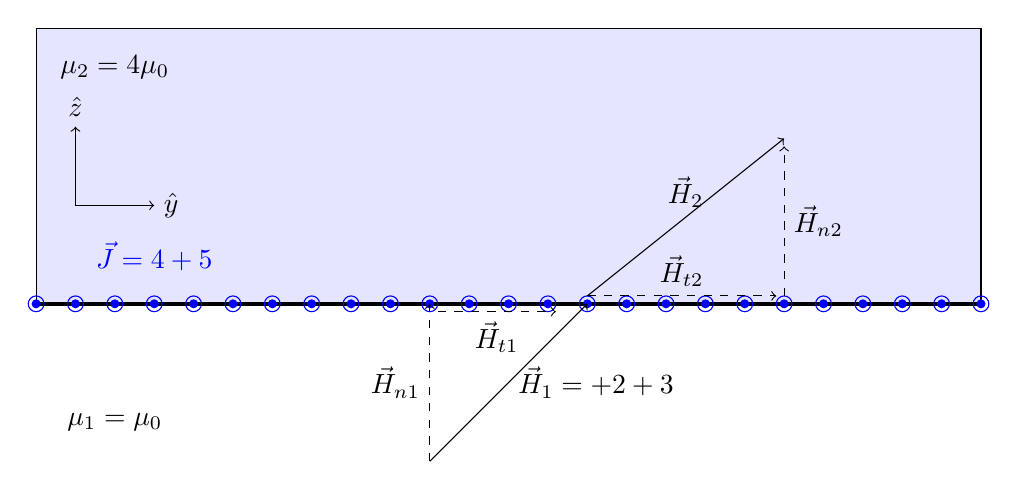
\begin{tikzpicture}

	\draw[fill=blue!10!white] (0,0) rectangle (12,3.5);
	\draw[ultra thick, black] (0,0) --++ (12,0);
	\node at (1,3) {$\mu_2 = 4\mu_0$};
	\node at (1,-1.5) {$\mu_1 = \mu_0$};
	
	% line charges
	\foreach \x in{0,0.5,1,...,12}{
		\draw[blue] (\x,0) circle (1mm);
		\draw[blue, fill=blue] (\x,0) circle (0.5mm);
%		\draw[green!50!black, ->] (\x+0.35,0) arc (0:315:0.3);
	}
	\node[blue] at (1.5,0.6) {$\vec{J} = \xhat 4 + \yhat 5$};
		
	% unit vectors
	\draw[->] (0.5,1.25) --++ (1,0) node[right] {$\hat{y}$};
	\draw[->] (0.5,1.25) --++ (0,1) node[above] {$\hat{z}$};
	
	% material 2
	\draw[->] (5,-2) --++ (2,2) node[midway, right] {$\vec{H}_1 = \xhat + \yhat 2 + \zhat 3$}; 
	\draw[->, dashed] (5,-2) --++ (0,2) node[left, midway] {$\vec{H}_{\text{n1}}$};
	\draw[->, dashed] (5.1,-0.1) --++ (1.5,0) node[below, midway] {$\vec{H}_{\text{t1}}$};
	
	% material 1
	\draw[->] (7, 0.1)  --++ (2.5,2) node[midway, above] {$\vec{H}_{2}$};
	\draw[->, dashed] (9.5, 0.1) --++ (0,1.9) node[right, midway] {$\vec{H}_{\text{n2}}$};
	\draw[->, dashed] (7,0.1) --++ (2.4,0) node[above, midway] {$\vec{H}_{\text{t2}}$};
	
\end{tikzpicture}
}% end scalebox
\end{textblock}
\begin{textblock}{7}(8.5,3)
\begin{scriptsize}
\eq{
	&\circled{1} \; \text{Draw a picture} \\
	&\circled{2} \; \text{Identify T \& N} \\
	&\qquad \vec{H}_{\text{t1}} = \handoutgap{0pt}{\xhat 1 + \yhat 2 \implies | \vec{H}_{\text{t1}} | = \sqrt{5} } \\
	&\qquad \vec{H}_{\text{n1}} = \handoutgap{0pt}{\yhat 3 \implies |\vec{H}_{\text{n1}}| = 3} \\
	&\circled{3}\; \hat{n}_{2,1} = \handoutgap{0pt}{-\zhat} \\
	&\circled{4} \; \text{Normal BC} \\
	&\handoutgap{0pt}{ \qquad \hat{n}_{21}\times\lp \vec{H}_1 - \vec{H}_2 \rp = \vec{J} }\\
	&\handoutgap{0pt}{\qquad -\zhat \times \lp \xhat + \yhat 2 + \zhat 3 \rp  }\\
	&\handoutgap{0pt}{\qquad - \lp -\zhat \rp \times\lp \xhat H_{2x} + \yhat H_{2y} + \zhat H_{2z} \rp = \vec{J}} \\
	&\handoutgap{0pt}{\qquad  -\yhat  + \xhat 2 +\yhat H_{2x} -\xhat H_{2y} = \xhat 4 + \yhat 5}\\
	&\handoutgap{0pt}{\qquad \xhat \lp 2 - H_{2y} \rp + \yhat \lp H_{2x} -1 \rp = \xhat 4 + \yhat 5 }\\
	&\;\implies H_{2y}  = \handoutgap{0pt}{-2}\\
	&\;\implies H_{2x} = \handoutgap{0pt}{6} \\ 	
} % end eq
\end{scriptsize}
\end{textblock}
\end{frame}

%%%%%%%%%%%%%%%%%%%%%%%%%%%%%%%%%%%%%%%%%%%%%%%%%%%%%%
%%%%%%%%%%%%%%%%%%%%%%%%%%%%%%%%%%%%%%%%%%%%%%%%%%%%%%
\begin{frame}{Boundary Condition: Example}
\begin{textblock}{7.5}(0.5,3)
A magnetic field $\vec{H} = \xhat + \yhat 2 + \zhat 3$ exists in a material with $\mu = \mu_0$ and is incident on a boundary with a surface current of $\vec{J} = \xhat 4 + \yhat 5$. The material on the other side of the boundary has $\mu = 4\mu_0$. Determine $\vec{H}_2$. 

\vspace{12pt} 

\scalebox{0.5}{
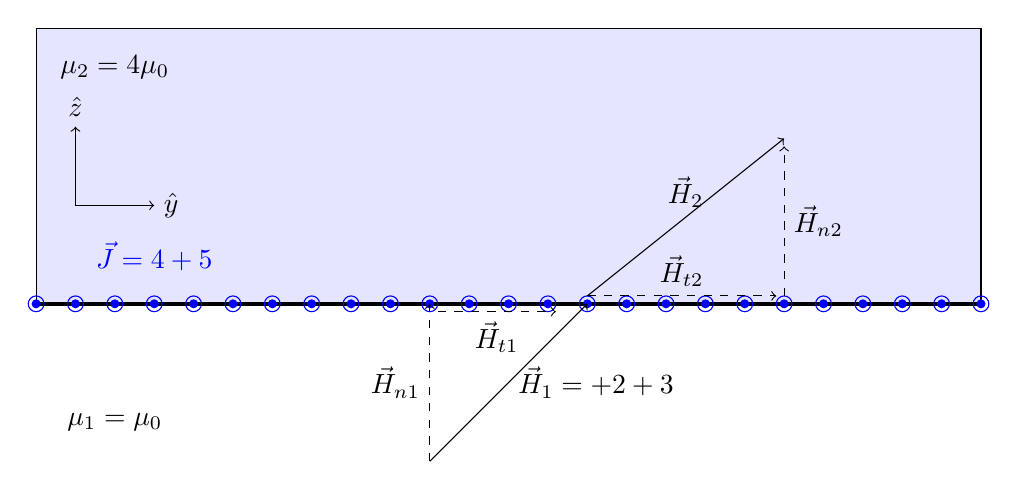
\begin{tikzpicture}

	\draw[fill=blue!10!white] (0,0) rectangle (12,3.5);
	\draw[ultra thick, black] (0,0) --++ (12,0);
	\node at (1,3) {$\mu_2 = 4\mu_0$};
	\node at (1,-1.5) {$\mu_1 = \mu_0$};
	
	% line charges
	\foreach \x in{0,0.5,1,...,12}{
		\draw[blue] (\x,0) circle (1mm);
		\draw[blue, fill=blue] (\x,0) circle (0.5mm);
%		\draw[green!50!black, ->] (\x+0.35,0) arc (0:315:0.3);
	}
	\node[blue] at (1.5,0.6) {$\vec{J} = \xhat 4 + \yhat 5$};
		
	% unit vectors
	\draw[->] (0.5,1.25) --++ (1,0) node[right] {$\hat{y}$};
	\draw[->] (0.5,1.25) --++ (0,1) node[above] {$\hat{z}$};
	
	% material 2
	\draw[->] (5,-2) --++ (2,2) node[midway, right] {$\vec{H}_1 = \xhat + \yhat 2 + \zhat 3$}; 
	\draw[->, dashed] (5,-2) --++ (0,2) node[left, midway] {$\vec{H}_{\text{n1}}$};
	\draw[->, dashed] (5.1,-0.1) --++ (1.5,0) node[below, midway] {$\vec{H}_{\text{t1}}$};
	
	% material 1
	\draw[->] (7, 0.1)  --++ (2.5,2) node[midway, above] {$\vec{H}_{2}$};
	\draw[->, dashed] (9.5, 0.1) --++ (0,1.9) node[right, midway] {$\vec{H}_{\text{n2}}$};
	\draw[->, dashed] (7,0.1) --++ (2.4,0) node[above, midway] {$\vec{H}_{\text{t2}}$};
	
\end{tikzpicture}
}% end scalebox
\end{textblock}
\begin{textblock}{7}(8.5,3)
\begin{scriptsize}
\eq{
	&\circled{5} \; \text{Normal BC} \\
	&\handoutgap{0pt}{\qquad \mu_1 H_{n1} = \mu_2 H_{n2} }\\
	&\handoutgap{0pt}{\qquad H_{2z} = \handoutgap{0pt}{\dfrac{\mu_0}{4\mu_0}3 = \dfrac{3}{4}}} \\
	&\circled{6} \; \text{Put it all together} \\
	&\qquad \vec{H}_2 = \handoutgap{0pt}{\xhat 6 -\yhat 2 + \zhat \dfrac{3}{4}} 
} % end eq
\end{scriptsize}
\end{textblock}
\end{frame}
